\documentclass[tikz,border=2pt]{standalone}
\usepackage{amsmath}
\usepackage{pgfplots}
\pgfplotsset{compat=1.18}
\usetikzlibrary{arrows.meta}
\begin{document}
% Closed halfspace S={x: x1+2x2<=4} with a=(1,2), b=4: the line H through (4,0) and (0,2) bounds S;
% a drawn from (4,0) to (5,2) points away from S; 0 in S, (2,2) not in S.
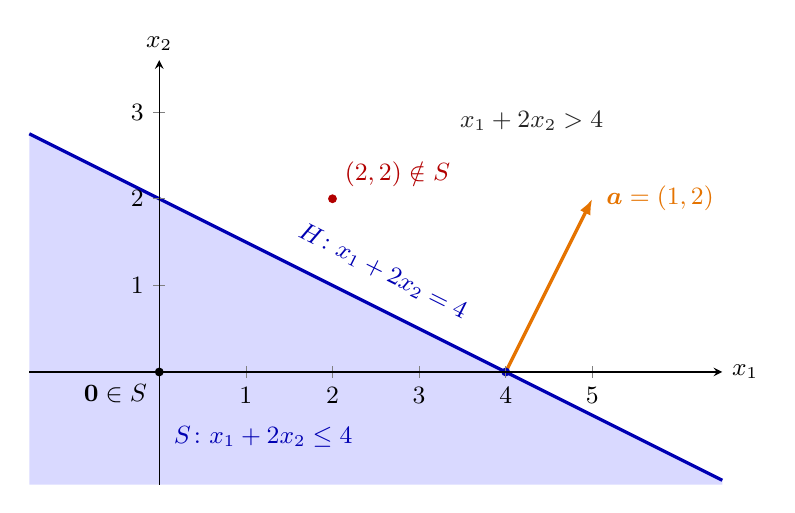
\begin{tikzpicture}[font=\small, >={Latex[length=2mm]}]
  \begin{axis}[
    axis lines=middle, xmin=-1.5, xmax=6.5, ymin=-1.3, ymax=3.6,
    xtick={1,2,3,4,5}, ytick={1,2,3}, axis on top,
    xlabel={$x_1$}, ylabel={$x_2$},
    xlabel style={anchor=west}, ylabel style={anchor=south},
    x=1.1cm, y=1.1cm, clip=false
    ]
    \fill[blue!15] (axis cs:-1.5,2.75) -- (axis cs:6.5,-1.25) -- (axis cs:6.5,-1.3) -- (axis cs:-1.5,-1.3) -- cycle;
    \draw[blue!70!black, very thick] (axis cs:-1.5,2.75) -- (axis cs:6.5,-1.25);
    \draw[orange!90!black, very thick, ->] (axis cs:4,0) -- (axis cs:5,2);
    \node[orange!90!black, anchor=west] at (axis cs:5.05,2) {$\boldsymbol{a}=(1,2)$};
    \fill[blue!70!black] (axis cs:4,0) circle (1.6pt);
    \fill (axis cs:0,0) circle (1.6pt);
    \node[anchor=north east] at (axis cs:-0.03,-0.03) {$\boldsymbol{0}\in S$};
    \fill[red!70!black] (axis cs:2,2) circle (1.6pt);
    \node[red!70!black, anchor=south west] at (axis cs:2.03,2.03) {$(2,2)\notin S$};
    \node[blue!70!black, anchor=south, rotate=-26.57] at (axis cs:2.48,0.96) {$H\colon x_1+2x_2=4$};
    \node[blue!70!black] at (axis cs:1.2,-0.75) {$S\colon x_1+2x_2\leq4$};
    \node[gray!30!black] at (axis cs:4.3,2.9) {$x_1+2x_2>4$};
  \end{axis}
\end{tikzpicture}
\end{document}
